\section{Xây dựng mô hình dự đoán}
\subsection{Các đại lượng đánh giá mô hình}
\label{subsec:evaluation_metrics_explanation}

Để đánh giá chất lượng và độ chính xác của các mô hình trong việc dự đoán sản lượng cây trồng, nhóm em sử dụng một tập hợp các đại lượng (metrics) đo lường phổ biến. Các đại lượng này giúp định lượng mức độ lỗi của mô hình cũng như khả năng giải thích sự biến thiên trong dữ liệu của mô hình. Dưới đây là giải thích chi tiết về từng đại lượng:

Trong các công thức dưới đây, chúng ta ký hiệu:
\begin{itemize}
    \item $n$: tổng số quan sát trong tập dữ liệu đánh giá (ví dụ: tập kiểm tra).
    \item $y_i$: giá trị thực tế của quan sát thứ $i$.
    \item $\hat{y}_i$: giá trị dự đoán bởi mô hình cho quan sát thứ $i$.
    \item $\bar{y}$: giá trị trung bình của các giá trị thực tế $y_i$, tức là $\bar{y} = \frac{1}{n} \sum_{i=1}^{n} y_i$.
\end{itemize}

\subsubsection{Mean Absolute Error (MAE) – Sai số Tuyệt đối trung bình}
\label{subsubsec:mae_explanation}
MAE đo lường độ lớn trung bình của các sai số trong một tập hợp các dự đoán, mà không xem xét đến chiều hướng của chúng. Đây là trung bình cộng của các chênh lệch tuyệt đối giữa giá trị dự đoán và giá trị thực tế.
\begin{equation}
    \text{MAE} = \frac{1}{n} \sum_{i=1}^{n} |y_i - \hat{y}_i|
    \label{eq:mae}
\end{equation}
\textbf{Ý nghĩa và diễn giải:}
\begin{itemize}
    \item MAE cho chúng ta biết, trung bình, dự đoán của mô hình lệch khỏi giá trị thực tế bao nhiêu đơn vị.
    \item Đơn vị của MAE giống với đơn vị của biến mục tiêu (ví dụ: nếu sản lượng tính bằng tấn/ha, MAE cũng sẽ có đơn vị là tấn/ha).
    \item Giá trị MAE càng gần 0, mô hình dự đoán càng chính xác.
    \item MAE không bị ảnh hưởng nhiều bởi các giá trị ngoại lệ (outliers) lớn như MSE vì nó không bình phương sai số.
\end{itemize}

\subsubsection{Mean Squared Error (MSE) – Sai số Bình phương trung bình}
\label{subsubsec:mse_explanation}
MSE là trung bình của bình phương các sai số, tức là chênh lệch giữa giá trị ước lượng và giá trị thực tế.
\begin{equation}
    \text{MSE} = \frac{1}{n} \sum_{i=1}^{n} (y_i - \hat{y}_i)^2
    \label{eq:mse}
\end{equation}
\textbf{Ý nghĩa và diễn giải:}
\begin{itemize}
    \item MSE nhấn mạnh các lỗi lớn hơn bằng cách bình phương chúng trước khi lấy trung bình. Do đó, một mô hình có MSE cao có thể là do có một vài dự đoán với sai số rất lớn.
    \item Đơn vị của MSE là bình phương của đơn vị biến mục tiêu (ví dụ: (tấn/ha)²), điều này làm cho việc diễn giải trực tiếp giá trị MSE trở nên khó khăn hơn so với MAE hoặc RMSE.
    \item Giá trị MSE càng gần 0, mô hình càng tốt.
    \item MSE thường được sử dụng trong các hàm mất mát (loss function) của nhiều thuật toán học máy do tính chất toán học thuận lợi của nó (ví dụ: khả vi).
\end{itemize}

\subsubsection{Root Mean Squared Error (RMSE) – Căn bậc hai Sai số Bình phương trung bình}
\label{subsubsec:rmse_explanation}
RMSE là căn bậc hai của MSE. Nó là một trong những đại lượng phổ biến nhất để đo lường sự khác biệt giữa các giá trị được dự đoán bởi một mô hình và các giá trị thực tế.
\begin{equation}
    \text{RMSE} = \sqrt{\text{MSE}} = \sqrt{\frac{1}{n} \sum_{i=1}^{n} (y_i - \hat{y}_i)^2}
    \label{eq:rmse}
\end{equation}
\textbf{Ý nghĩa và diễn giải:}
\begin{itemize}
    \item RMSE có cùng đơn vị với biến mục tiêu (giống như MAE), giúp việc diễn giải trở nên trực quan hơn so với MSE. Ví dụ, nếu RMSE là 0.5 tấn/ha, điều này có nghĩa là độ lệch chuẩn của các phần dư (sai số dự đoán) là 0.5 tấn/ha.
    \item Tương tự MSE, RMSE cũng nhạy cảm với các giá trị ngoại lệ do việc bình phương sai số. Các lỗi lớn sẽ làm tăng RMSE một cách đáng kể.
    \item Giá trị RMSE càng gần 0, mô hình dự đoán càng chính xác.
    \item Khi so sánh hai mô hình, mô hình có RMSE thấp hơn thường được coi là tốt hơn (giả sử các yếu tố khác là tương đương).
\end{itemize}

\subsubsection{R-squared (R²) – Hệ số xác định}
\label{subsubsec:r_squared_explanation}
R-squared, hay còn gọi là hệ số xác định, là một đại lượng thống kê đo lường tỷ lệ phần trăm phương sai (variance) của biến phụ thuộc (biến mục tiêu) mà mô hình hồi quy có thể giải thích được. Nói cách khác, nó cho biết mức độ phù hợp của mô hình với dữ liệu quan sát được.
\begin{equation}
    R^2 = 1 - \frac{SS_{\text{res}}}{SS_{\text{tot}}} = 1 - \frac{\sum_{i=1}^{n} (y_i - \hat{y}_i)^2}{\sum_{i=1}^{n} (y_i - \bar{y})^2}
    \label{eq:r_squared}
\end{equation}
Trong đó:
\begin{itemize}
    \item $SS_{\text{res}} = \sum_{i=1}^{n} (y_i - \hat{y}_i)^2$ là tổng bình phương các phần dư (Residual Sum of Squares), đo lường phần phương sai không giải thích được bởi mô hình.
    \item $SS_{\text{tot}} = \sum_{i=1}^{n} (y_i - \bar{y})^2$ là tổng bình phương toàn phần (Total Sum of Squares), đo lường tổng phương sai của biến mục tiêu.
\end{itemize}
\textbf{Ý nghĩa và diễn giải:}
\begin{itemize}
    \item $R^2$ có giá trị nằm trong khoảng từ $-\infty$ đến $1$. Tuy nhiên, trong hầu hết các trường hợp thực tế với các mô hình hợp lý, $R^2$ sẽ nằm trong khoảng từ $0$ đến $1$.
    \item $R^2 = 1$: Mô hình giải thích được toàn bộ sự biến thiên trong dữ liệu, tức là các giá trị dự đoán hoàn toàn khớp với giá trị thực tế. Đây là trường hợp lý tưởng nhưng hiếm khi xảy ra.
    \item $R^2 = 0$: Mô hình không giải thích được chút nào sự biến thiên trong dữ liệu. Mô hình dự đoán không tốt hơn việc chỉ sử dụng giá trị trung bình $\bar{y}$ để dự đoán cho tất cả các quan sát.
    \item $R^2 > 0$: Ví dụ, $R^2 = 0.75$ có nghĩa là $75\%$ sự biến thiên của biến mục tiêu được giải thích bởi các biến độc lập trong mô hình. $25\%$ còn lại là do các yếu tố khác không được mô hình nắm bắt.
    \item $R^2 < 0$: Điều này có thể xảy ra nếu mô hình dự đoán tệ hơn cả việc chỉ dùng giá trị trung bình $\bar{y}$. Thường gặp khi mô hình được chọn không phù hợp với dữ liệu.
    \item Giá trị $R^2$ càng gần $1$ thì mô hình càng phù hợp với dữ liệu. Tuy nhiên, một $R^2$ cao không phải lúc nào cũng đồng nghĩa với một mô hình tốt. Việc thêm quá nhiều biến vào mô hình (ngay cả những biến không liên quan) có thể làm tăng $R^2$ một cách giả tạo. Do đó, $R^2$ nên được xem xét cùng với các chỉ số khác và bối cảnh của bài toán. Adjusted R-squared (R² điều chỉnh) là một biến thể thường được sử dụng để khắc phục nhược điểm này bằng cách phạt việc thêm các biến không cần thiết.
\end{itemize}

Việc hiểu rõ ý nghĩa của từng đại lượng đánh giá này giúp chúng ta có cái nhìn toàn diện hơn về hiệu suất của các mô hình hồi quy và đưa ra những quyết định tốt hơn trong việc lựa chọn và cải tiến mô hình.






\subsection{Mô hình Hồi quy tuyến tính}
\label{subsec:linear_regression_results}

Sau khi xây dựng và huấn luyện mô hình Hồi quy Tuyến tính sử dụng các đặc trưng về thời tiết, nông nghiệp và các yếu tố khác (bao gồm các biến phân loại đã được mã hóa bằng One-Hot Encoding) để dự đoán sản lượng cây trồng (`Crop\_Yield\_MT\_per\_HA`), nhóm em đã thu được các kết quả đánh giá và hệ số như sau. 

\subsubsection{Các chỉ số đánh giá hiệu suất mô hình}
\label{subsubsec:lr_performance_metrics}

Hiệu suất của mô hình Hồi quy Tuyến tính trên tập kiểm tra được đánh giá thông qua các chỉ số sau:
\begin{itemize}
    \item \textbf{Mean Absolute Error (MAE):} $0.5466$
    \item \textbf{Mean Squared Error (MSE):} $0.4648$
    \item \textbf{Root Mean Squared Error (RMSE):} $0.6818$
    \item \textbf{R-squared (R²):} $0.5596$
\end{itemize}
Hệ số chặn (Intercept) của mô hình là $-0.6208$.

Giá trị $R^2 = 0.5596$ cho thấy mô hình Hồi quy Tuyến tính của nhóm em giải thích được khoảng $55.96\%$ sự biến thiên của sản lượng cây trồng. Đây là một mức độ giải thích ở mức khá, chỉ ra rằng các đặc trưng được lựa chọn có vai trò nhất định trong việc dự đoán sản lượng. Tuy nhiên, cũng có nghĩa là còn khoảng $44\%$ sự biến thiên của sản lượng chưa được mô hình nắm bắt, có thể do các yếu tố khác không được đưa vào mô hình hoặc do mối quan hệ phi tuyến tính phức tạp hơn.

Các chỉ số sai số MAE ($0.5466$) và RMSE ($0.6818$) cho biết mức độ lỗi trung bình của dự đoán so với giá trị thực tế (đơn vị là tấn/ha, giả sử sản lượng được đo bằng đơn vị này). Ví dụ, RMSE là $0.6818$ tấn/ha ngụ ý rằng, trung bình, các dự đoán của mô hình có thể lệch khoảng $0.68$ tấn/ha so với sản lượng thực tế. Mức độ sai số này cần được xem xét trong bối cảnh giá trị trung bình và độ biến động chung của sản lượng cây trồng trong bộ dữ liệu.

\subsubsection{Phân tích các hệ số hồi quy}
\label{subsubsec:lr_coefficients}

Các hệ số hồi quy ước lượng mức độ ảnh hưởng của mỗi đặc trưng đến sản lượng cây trồng, khi các yếu tố khác được giữ không đổi. Dưới đây là một số hệ số nổi bật từ mô hình (đã được sắp xếp theo giá trị tuyệt đối giảm dần từ file \texttt{regression\_coefficients.csv}):

\begin{itemize}
    \item \texttt{Crop\_Type\_Rice}: $2.2917$
    \item \texttt{Crop\_Type\_Wheat}: $-1.3206$
    \item \texttt{Crop\_Type\_Soybeans}: $-1.0568$
    \item \texttt{Fertilizer\_Use\_KG\_per\_HA}: $0.8000$
    \item \texttt{Adaptation\_Strategies\_Water Management}: $-0.7121$
\end{itemize}

Từ các hệ số này, có thể rút ra một số nhận xét sơ bộ:
\begin{itemize}
    \item Việc trồng lúa (\texttt{Crop\_Type\_Rice}) có hệ số dương lớn nhất ($2.2917$), cho thấy loại cây này có sản lượng dự kiến cao hơn đáng kể so với loại cây tham chiếu (sau khi One-Hot Encoding). Ngược lại, lúa mì (\texttt{Crop\_Type\_Wheat}) và đậu nành (\texttt{Crop\_Type\_Soybeans}) có hệ số âm, ngụ ý sản lượng dự kiến thấp hơn.
    \item Lượng phân bón sử dụng (\texttt{Fertilizer\_Use\_KG\_per\_HA}) có hệ số dương ($0.8000$), điều này phù hợp với kỳ vọng rằng việc tăng cường sử dụng phân bón (trong một chừng mực nhất định) sẽ giúp tăng sản lượng.
    \item Chiến lược thích ứng về quản lý nước (\texttt{Adaptation\_Strategies\_Water Management}) có hệ số âm ($-0.7121$). Điều này có vẻ phản trực giác và cần được phân tích sâu hơn. Có thể các khu vực áp dụng chiến lược này vốn dĩ đã gặp vấn đề nghiêm trọng về nước, hoặc chiến lược này chưa thực sự hiệu quả trong bối cảnh dữ liệu thu thập được, hoặc nó tương quan với các yếu tố khác làm giảm sản lượng.
\end{itemize}
Cần lưu ý rằng đây là các diễn giải ban đầu và mối quan hệ thực tế có thể phức tạp hơn do tương tác giữa các biến. Toàn bộ danh sách các hệ số được lưu trong file \texttt{regression\_coefficients.csv} tại thư mục kết quả.

\subsubsection{Trực quan hóa kết quả}
\label{subsubsec:lr_visualization}

Để đánh giá trực quan hơn về hiệu suất của mô hình, nhóm em xem xét hai biểu đồ chính: biểu đồ so sánh giá trị sản lượng thực tế và dự đoán (Hình \ref{fig:lr_actual_vs_predicted}), và biểu đồ phân phối của phần dư (Hình \ref{fig:lr_residuals_distribution}).

\begin{figure}[htb]
    \centering
    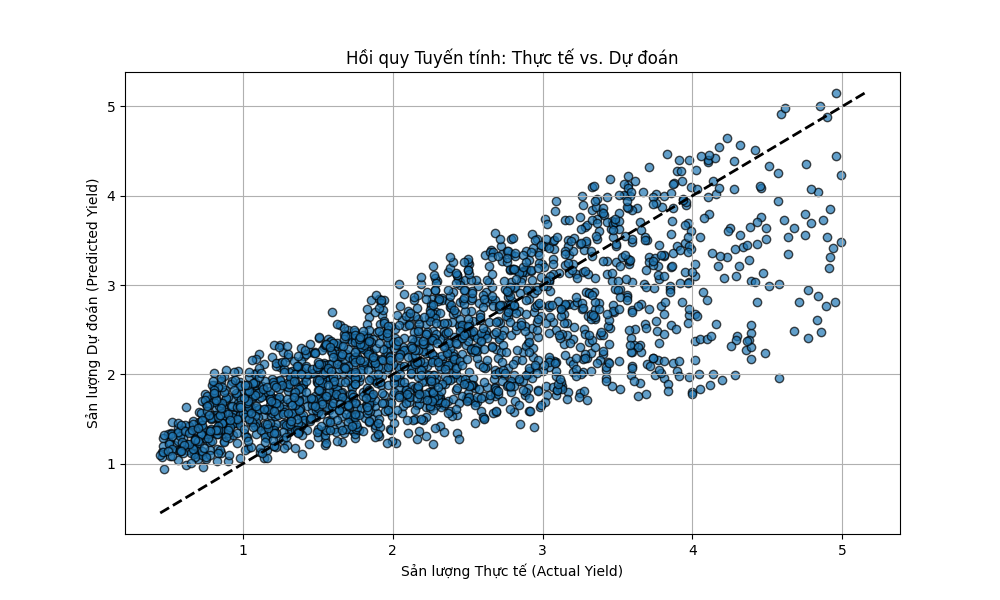
\includegraphics[width=0.9\textwidth]{Images/actual_vs_predicted_plot.png} 
    \caption{So sánh giá trị sản lượng thực tế và giá trị dự đoán bởi mô hình Hồi quy Tuyến tính trên tập kiểm tra.}
    \vspace{10pt}
    \label{fig:lr_actual_vs_predicted}
\end{figure}
\FloatBarrier
Hình \ref{fig:lr_actual_vs_predicted} cho thấy các điểm dữ liệu (mỗi điểm tương ứng với một quan sát trong tập kiểm tra) phân bố quanh đường chéo $y=x$. Nếu các điểm nằm hoàn toàn trên đường này, mô hình sẽ dự đoán chính xác tuyệt đối. Trong trường hợp này, các điểm có xu hướng bám theo đường chéo, nhưng cũng có sự phân tán nhất định, phản ánh các sai số MAE và RMSE đã tính toán ở trên. Điều này cho thấy mô hình nắm bắt được xu hướng chung nhưng vẫn còn những dự đoán chưa hoàn toàn chính xác.

\begin{figure}[htb]
    \centering
    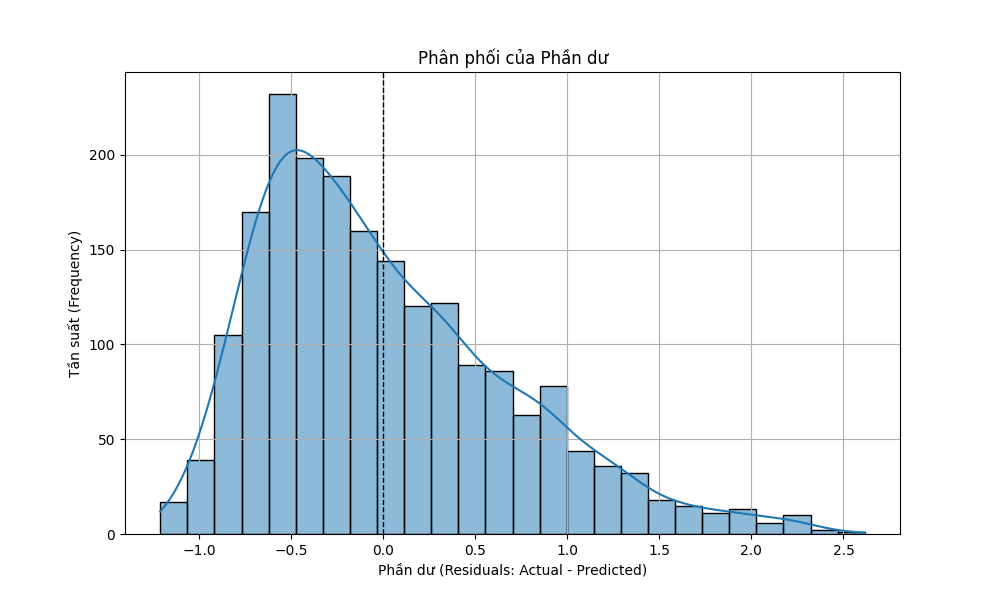
\includegraphics[width=0.9\textwidth]{Images/residuals_distribution_plot.png} 
    \vspace{10pt}
    \caption{Phân phối của phần dư (Actual - Predicted) từ mô hình Hồi quy Tuyến tính trên tập kiểm tra.}
    \label{fig:lr_residuals_distribution}
\end{figure}
\FloatBarrier
Hình \ref{fig:lr_residuals_distribution} thể hiện phân phối của phần dư (sai số giữa giá trị thực tế và giá trị dự đoán). Một mô hình tốt thường có phần dư phân phối chuẩn với giá trị trung bình gần bằng 0 và không có hình mẫu rõ ràng khi vẽ theo giá trị dự đoán (điều này không được hiển thị ở đây nhưng là một phần của phân tích phần dư sâu hơn). Trong biểu đồ này, phần dư có vẻ tập trung quanh 0 và có hình dạng gần giống phân phối chuông, điều này là một dấu hiệu tích cực, cho thấy mô hình không có thiên lệch hệ thống (systematic bias) rõ rệt. Tuy nhiên, sự tồn tại của một số phần dư có giá trị lớn (ở hai phía của đuôi phân phối) cũng chỉ ra các trường hợp mà mô hình dự đoán kém chính xác.

\subsubsection{Tóm tắt và Nhận xét}
Mô hình Hồi quy Tuyến tính đã cung cấp một cái nhìn ban đầu về mối quan hệ giữa các yếu tố đầu vào và sản lượng nông nghiệp. Với $R^2 \approx 0.56$, mô hình có khả năng giải thích một phần đáng kể sự biến động của sản lượng. Các hệ số cung cấp thông tin về hướng và cường độ tương đối của các yếu tố. Tuy nhiên, mức độ sai số và phần $R^2$ còn lại cho thấy tiềm năng cải thiện bằng cách sử dụng các mô hình phức tạp hơn, kỹ thuật đặc trưng tiên tiến hơn, hoặc thu thập thêm dữ liệu/đặc trưng có liên quan.





\subsection{ Mô hình Cây Quyết định (Decision Tree Regressor)}
\label{subsec:decision_tree_results}

Tiếp theo mô hình Hồi quy Tuyến tính, nhóm em đã xây dựng và đánh giá một mô hình Cây Quyết định (Decision Tree Regressor) để dự đoán sản lượng cây trồng (`Crop\_Yield\_MT\_per\_HA`). Mô hình này sử dụng các đặc trưng tương tự như mô hình hồi quy, bao gồm các biến đã được mã hóa One-Hot.

\subsubsection{Các chỉ số đánh giá hiệu suất mô hình}
\label{subsubsec:dt_performance_metrics}

Hiệu suất của mô hình Cây Quyết định trên tập kiểm tra được đánh giá như sau:
\begin{itemize}
    \item \textbf{Mean Absolute Error (MAE):} $0.6705$
    \item \textbf{Mean Squared Error (MSE):} $0.7727$
    \item \textbf{Root Mean Squared Error (RMSE):} $0.8791$
    \item \textbf{R-squared (R²):} $0.2679$
\end{itemize}

Giá trị $R^2 = 0.2679$ cho thấy mô hình Cây Quyết định (với các tham số mặc định) giải thích được khoảng $26.79\%$ sự biến thiên của sản lượng cây trồng. Con số này thấp hơn đáng kể so với mô hình Hồi quy Tuyến tính ($R^2 \approx 0.56$). Điều này gợi ý rằng mô hình Cây Quyết định cơ bản có thể chưa nắm bắt tốt các mối quan hệ trong dữ liệu, hoặc có thể đang bị hiện tượng overfitting (học quá khớp trên tập huấn luyện) hoặc underfitting nếu cây quá nông.

Các chỉ số sai số MAE ($0.6705$) và RMSE ($0.8791$) cũng cao hơn so với mô hình Hồi quy Tuyến tính, cho thấy dự đoán của mô hình Cây Quyết định này, trung bình, lệch nhiều hơn so với giá trị sản lượng thực tế.

\subsubsection{Phân tích độ quan trọng của các đặc trưng (Feature Importances)}
\label{subsubsec:dt_feature_importances}

Khác với Hồi quy Tuyến tính sử dụng hệ số, Cây Quyết định đánh giá tầm quan trọng của các đặc trưng dựa trên mức độ chúng đóng góp vào việc giảm thiểu sai số (hoặc tạp chất) tại các nút chia của cây. Dưới đây là 5 đặc trưng có độ quan trọng cao nhất theo mô hình (từ file \texttt{dt\_feature\_importances.csv}):

\begin{enumerate}
    \item \texttt{Fertilizer\_Use\_KG\_per\_HA}: $0.5360$
    \item \texttt{Crop\_Type\_Rice}: $0.1608$
    \item \texttt{Year}: $0.0616$
    \item \texttt{Pesticide\_Use\_KG\_per\_HA}: $0.0400$
    \item \texttt{Soil\_Health\_Index}: $0.0331$
\end{enumerate}

Nhận xét từ các đặc trưng quan trọng nhất:
\begin{itemize}
    \item Lượng phân bón sử dụng (\texttt{Fertilizer\_Use\_KG\_per\_HA}) là đặc trưng có ảnh hưởng lớn nhất đến các quyết định của cây, chiếm tới hơn $53\%$ tổng độ quan trọng. Điều này nhấn mạnh vai trò then chốt của phân bón trong mô hình dự đoán sản lượng này.
    \item Việc trồng lúa (\texttt{Crop\_Type\_Rice}) cũng là một yếu tố quan trọng ($16.08\%$).
    \item Năm (\texttt{Year}), lượng thuốc trừ sâu (\texttt{Pesticide\_Use\_KG\_per\_HA}), và chỉ số sức khỏe đất (\texttt{Soil\_Health\_Index}) cũng có những đóng góp đáng kể, mặc dù ở mức độ thấp hơn.
\end{itemize}
Việc các đặc trưng liên quan đến loại cây trồng và yếu tố đầu vào nông nghiệp (phân bón, thuốc trừ sâu) có độ quan trọng cao là điều dễ hiểu. Độ quan trọng của `Year` có thể phản ánh xu hướng thay đổi sản lượng theo thời gian do các yếu tố không được đo lường trực tiếp khác (ví dụ: cải tiến công nghệ, chính sách nông nghiệp).

\subsubsection{Trực quan hóa kết quả và cấu trúc cây}
\label{subsubsec:dt_visualization}

Các biểu đồ sau giúp đánh giá trực quan hiệu suất và cấu trúc của mô hình Cây Quyết định.

\begin{figure}[htb]
    \centering
    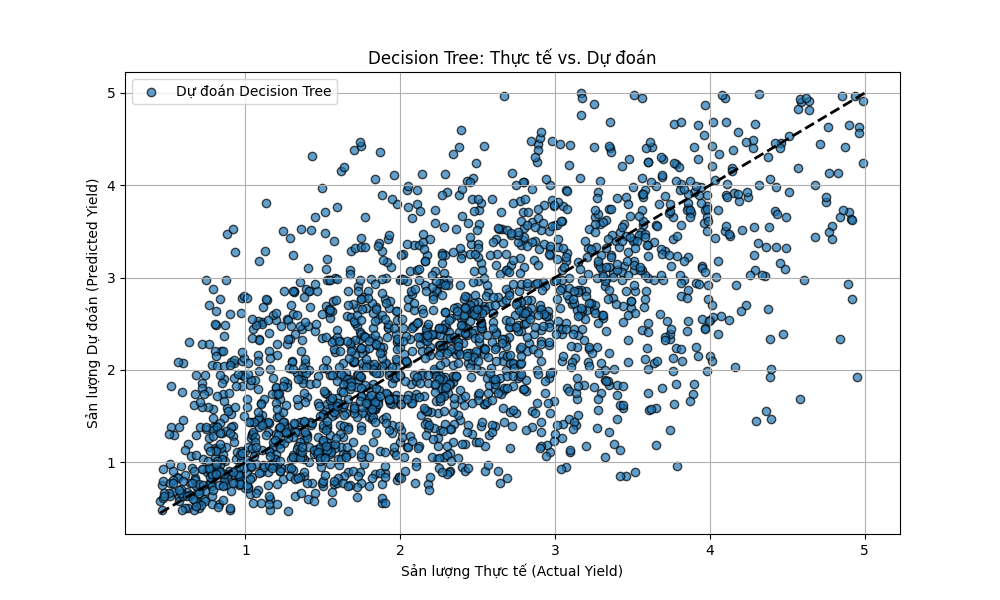
\includegraphics[width=0.8\textwidth]{Images/dt_actual_vs_predicted_plot.png} % ĐIỀU CHỈNH ĐƯỜNG DẪN
    \caption{So sánh giá trị sản lượng thực tế và giá trị dự đoán bởi mô hình Cây Quyết định trên tập kiểm tra.}
    \label{fig:dt_actual_vs_predicted}
\end{figure}

Hình \ref{fig:dt_actual_vs_predicted} cho thấy sự phân tán của các điểm dự đoán so với giá trị thực tế. So với mô hình Hồi quy Tuyến tính, các điểm có vẻ phân tán rộng hơn so với đường chéo $y=x$, điều này cũng phù hợp với giá trị $R^2$ thấp hơn và các chỉ số lỗi cao hơn. Có thể thấy một số cụm điểm dự đoán nằm trên các đường ngang, đây là đặc điểm của Cây Quyết định khi các mẫu rơi vào cùng một nút lá sẽ có cùng một giá trị dự đoán.

\begin{figure}[htb]
    \centering
    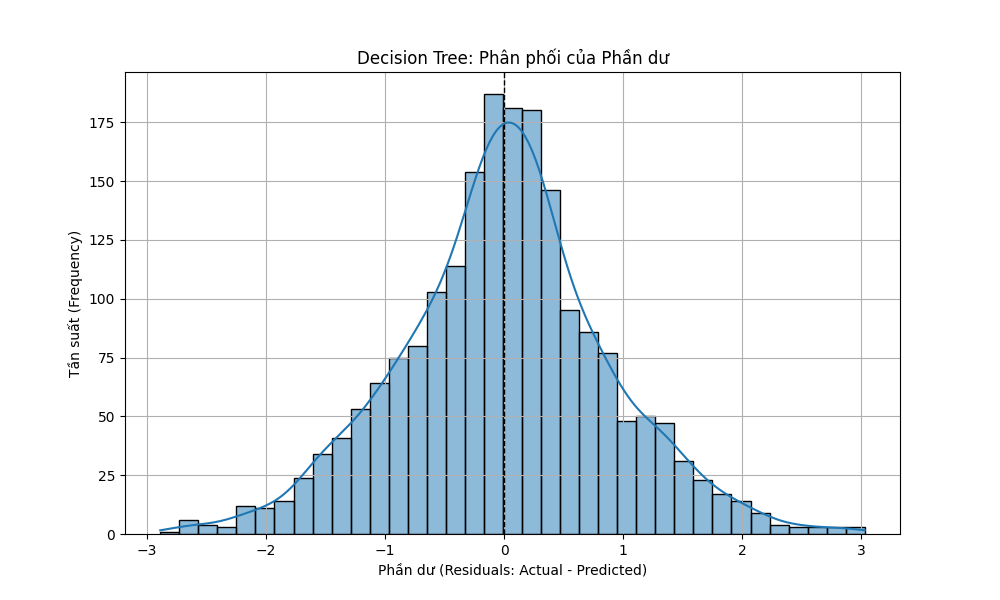
\includegraphics[width=0.8\textwidth]{Images/dt_residuals_distribution_plot.png} 
    \caption{Phân phối của phần dư (Actual - Predicted) từ mô hình Cây Quyết định trên tập kiểm tra.}
    \label{fig:dt_residuals_distribution}
\end{figure}

Phân phối phần dư (Hình \ref{fig:dt_residuals_distribution}) của mô hình Cây Quyết định cũng tập trung quanh 0, nhưng có vẻ rộng hơn và không đối xứng bằng so với mô hình Hồi quy Tuyến tính. Điều này cũng củng cố nhận định rằng mô hình Cây Quyết định (với tham số mặc định) có hiệu suất kém hơn trong trường hợp này.

\begin{figure}[htb]
    \centering
    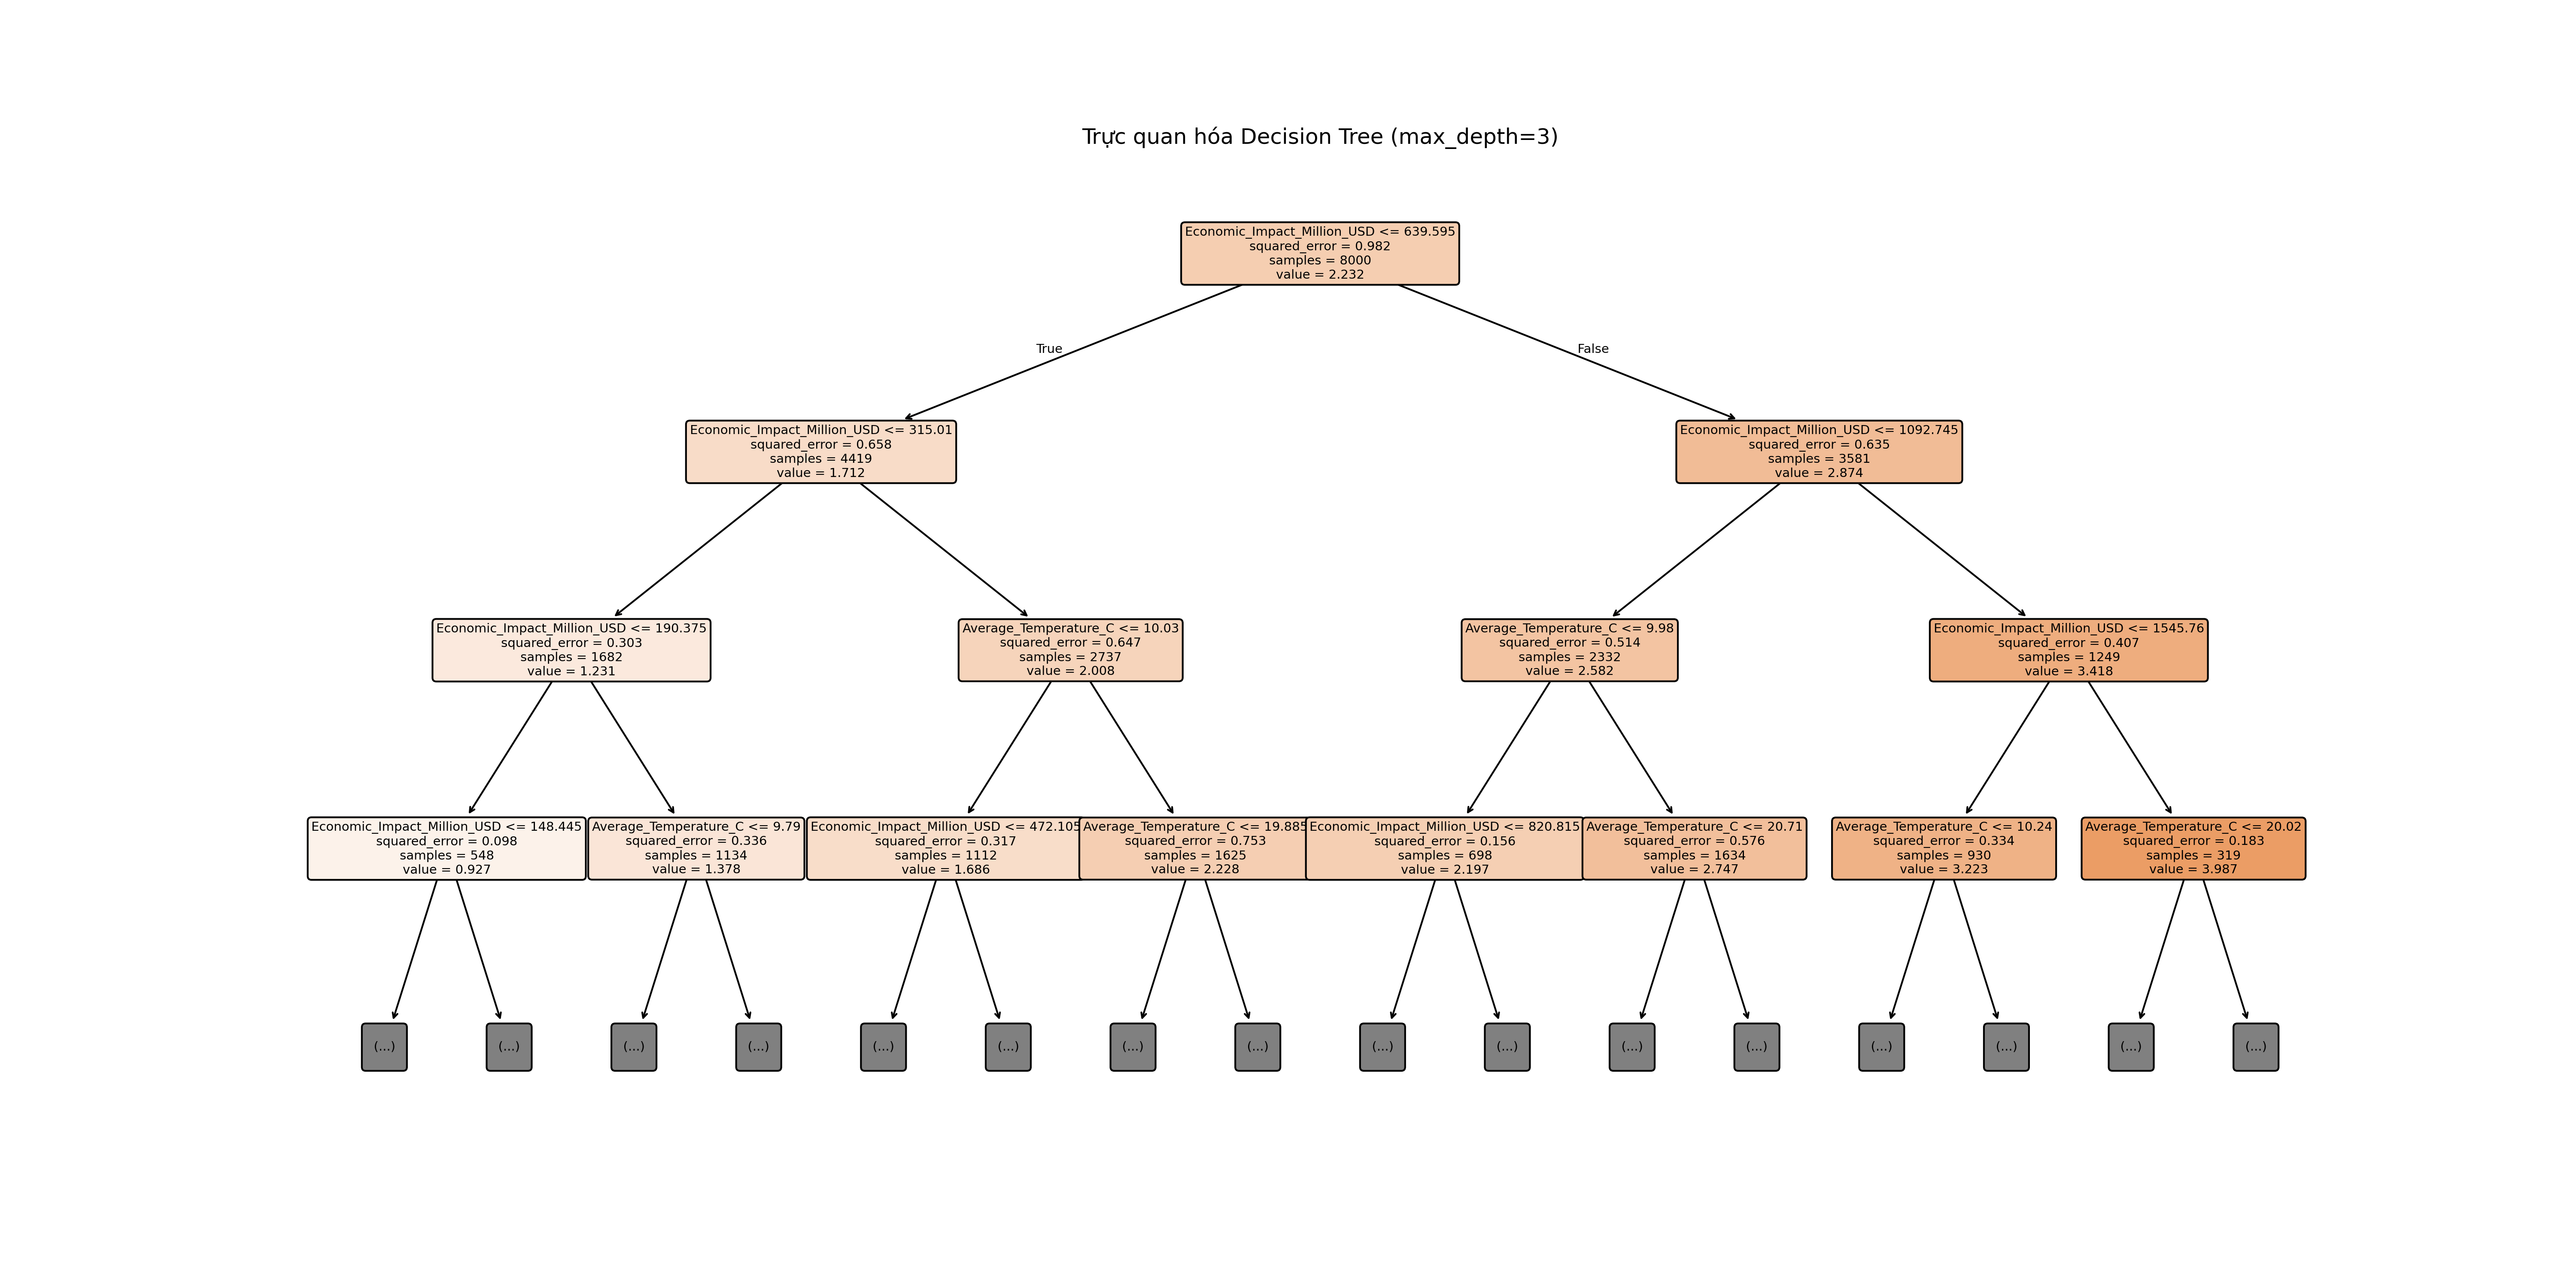
\includegraphics[width=0.9\textwidth]{Images/dt_tree_visualization.png} 
    \caption{Trực quan hóa 3 tầng đầu tiên của mô hình Cây Quyết định. Các nút hiển thị điều kiện chia, giá trị mse, số lượng mẫu (samples) và giá trị dự đoán trung bình (value) tại nút đó.}
    \label{fig:dt_tree_visualization}
\end{figure}

Hình \ref{fig:dt_tree_visualization} minh họa cấu trúc của 3 tầng đầu tiên trong cây quyết định đã huấn luyện. Tại mỗi nút, cây đưa ra một quyết định dựa trên một đặc trưng và một ngưỡng giá trị để chia dữ liệu. Ví dụ, ở nút gốc (tầng trên cùng), cây có thể chia dựa trên \texttt{Fertilizer\_Use\_KG\_per\_HA}. Các mẫu dữ liệu sau đó sẽ đi theo các nhánh tương ứng dựa trên việc chúng thỏa mãn điều kiện chia hay không. Giá trị `value` tại mỗi nút lá (hoặc nút trung gian) là giá trị sản lượng trung bình của các mẫu thuộc về nút đó. Biểu đồ này giúp hiểu rõ hơn cách mô hình đưa ra dự đoán, dù chỉ là một phần nhỏ của cây đầy đủ.

\subsubsection{Tóm tắt và Nhận xét}
Mô hình Cây Quyết định với các tham số mặc định cho thấy hiệu suất dự đoán sản lượng nông nghiệp thấp hơn so với mô hình Hồi quy Tuyến tính trong nghiên cứu này, thể hiện qua chỉ số $R^2$ thấp hơn và các lỗi MAE, RMSE cao hơn. Đặc trưng quan trọng nhất được xác định là lượng phân bón sử dụng.
Dù vậy, việc phân tích độ quan trọng của đặc trưng và trực quan hóa cây cũng cung cấp những hiểu biết giá trị về dữ liệu.








\subsection{ Mô hình Mạng Nơ-ron Nhân tạo (ANN - MLPRegressor)}
\label{subsec:ann_results}

Để khám phá khả năng của các mô hình phức tạp hơn trong việc nắm bắt các mối quan hệ phi tuyến tiềm ẩn trong dữ liệu, nhóm em đã triển khai một Mạng Nơ-ron Nhân tạo dạng Multi-layer Perceptron Regressor (MLPRegressor). Một bước tiền xử lý quan trọng cho ANN là chuẩn hóa đặc trưng (feature scaling), do đó tất cả các đặc trưng đầu vào đã được chuẩn hóa bằng \texttt{StandardScaler} trước khi đưa vào mô hình. 

\subsubsection{Thông số và Kiến trúc Mô hình ANN}
\label{subsubsec:ann_architecture_metrics}

Mô hình MLPRegressor được cấu hình với các tham số chính như sau:
\begin{itemize}
    \item \textbf{Kiến trúc lớp ẩn (hidden\_layer\_sizes):} (100, 50) - bao gồm 2 lớp ẩn, lớp thứ nhất có 100 nơ-ron và lớp thứ hai có 50 nơ-ron.
    \item \textbf{Hàm kích hoạt (activation function):} ReLU (\texttt{relu}).
    \item \textbf{Thuật toán tối ưu (solver):} Adam (\texttt{adam}).
    \item \textbf{Số vòng lặp tối đa (max\_iter):} 500.
    \item \textbf{Dừng sớm (early\_stopping):} Được kích hoạt. Mô hình thực tế đã dừng sau 22 vòng lặp do không có sự cải thiện đáng kể trên tập validation.
\end{itemize}

Hiệu suất của mô hình ANN trên tập kiểm tra được đánh giá qua các chỉ số:
\begin{itemize}
    \item \textbf{Mean Absolute Error (MAE):} $0.5614$
    \item \textbf{Mean Squared Error (MSE):} $0.5047$
    \item \textbf{Root Mean Squared Error (RMSE):} $0.7104$
    \item \textbf{R-squared (R²):} $0.5218$
\end{itemize}

Giá trị $R^2 = 0.5218$ cho thấy mô hình ANN (với cấu hình ban đầu này) giải thích được khoảng $52.18\%$ sự biến thiên của sản lượng cây trồng. Kết quả này thấp hơn một chút so với mô hình Hồi quy Tuyến tính ($R^2 \approx 0.56$) nhưng cao hơn đáng kể so với mô hình Cây Quyết định với các tham số mặc định ($R^2 \approx 0.27$). Điều này cho thấy tiềm năng của ANN, tuy nhiên hiệu suất có thể được cải thiện thêm thông qua việc tinh chỉnh sâu hơn các siêu tham số và kiến trúc mạng.

Các chỉ số sai số MAE ($0.5614$) và RMSE ($0.7104$) cũng phản ánh mức độ lỗi tương tự như mô hình Hồi quy Tuyến tính.

\subsubsection{Trực quan hóa kết quả và quá trình huấn luyện}
\label{subsubsec:ann_visualization}

Ba biểu đồ chính được sử dụng để đánh giá mô hình ANN:

\begin{figure}[htb]
    \centering
    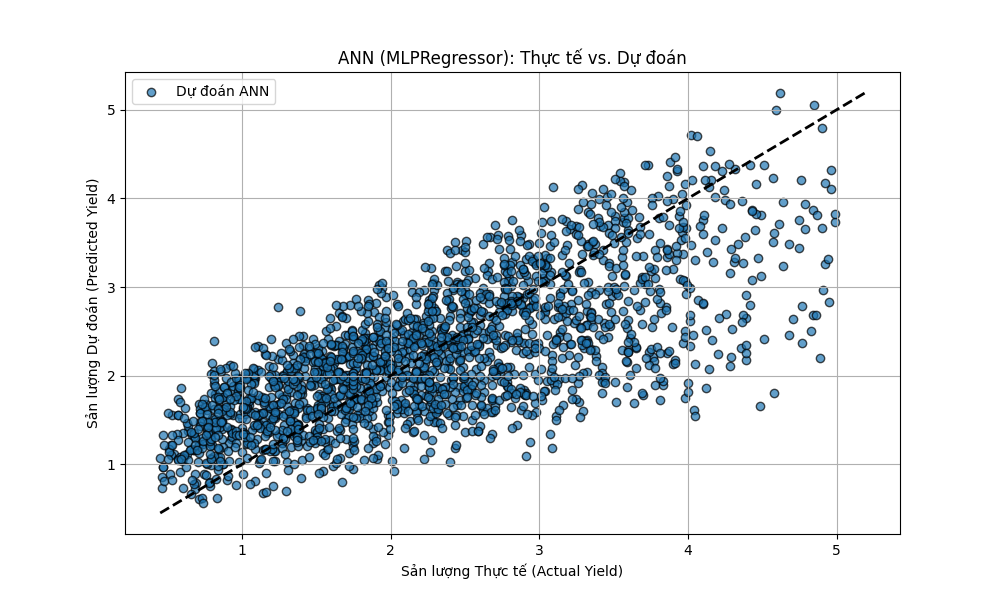
\includegraphics[width=0.8\textwidth]{Images/ann_actual_vs_predicted_plot.png}
    \caption{So sánh giá trị sản lượng thực tế và giá trị dự đoán bởi mô hình ANN trên tập kiểm tra.}
    \label{fig:ann_actual_vs_predicted}
\end{figure}
\FloatBarrier
Hình \ref{fig:ann_actual_vs_predicted} minh họa sự tương quan giữa giá trị sản lượng thực tế và giá trị dự đoán. Tương tự như mô hình Hồi quy Tuyến tính, các điểm dữ liệu có xu hướng tập trung quanh đường chéo $y=x$, cho thấy mô hình có khả năng dự đoán nhất định. Sự phân tán của các điểm phản ánh mức độ sai số của mô hình.

\begin{figure}[htb]
    \centering
    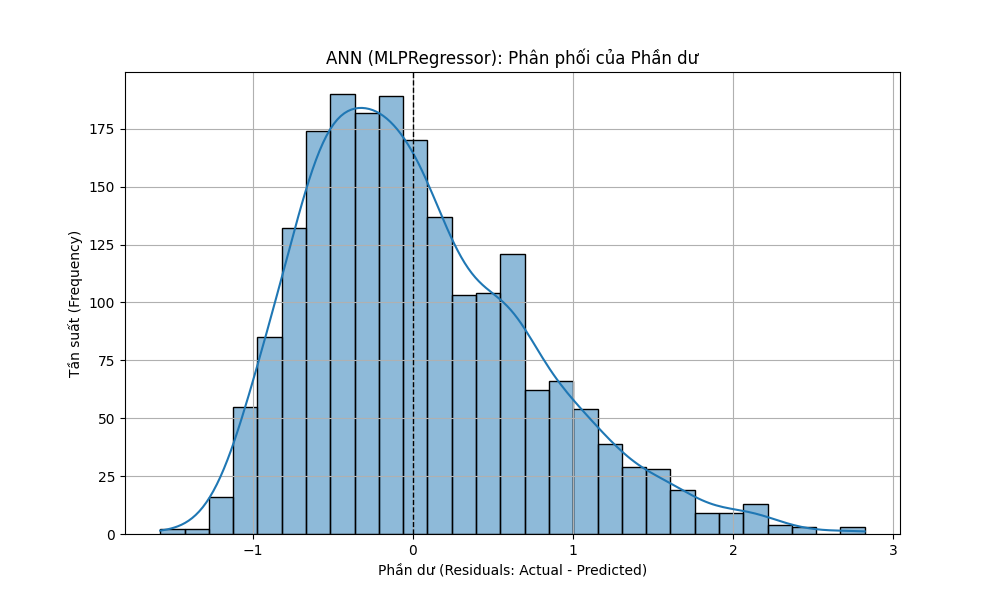
\includegraphics[width=0.8\textwidth]{Images/ann_residuals_distribution_plot.png} 
    \caption{Phân phối của phần dư (Actual - Predicted) từ mô hình ANN trên tập kiểm tra.}
    \label{fig:ann_residuals_distribution}
\end{figure}
\FloatBarrier
Phân phối phần dư của mô hình ANN (Hình \ref{fig:ann_residuals_distribution}) cũng tập trung quanh giá trị 0 và có hình dạng gần đối xứng, gợi ý rằng mô hình không mắc phải lỗi thiên lệch hệ thống nghiêm trọng.

\begin{figure}[htb]
    \centering
    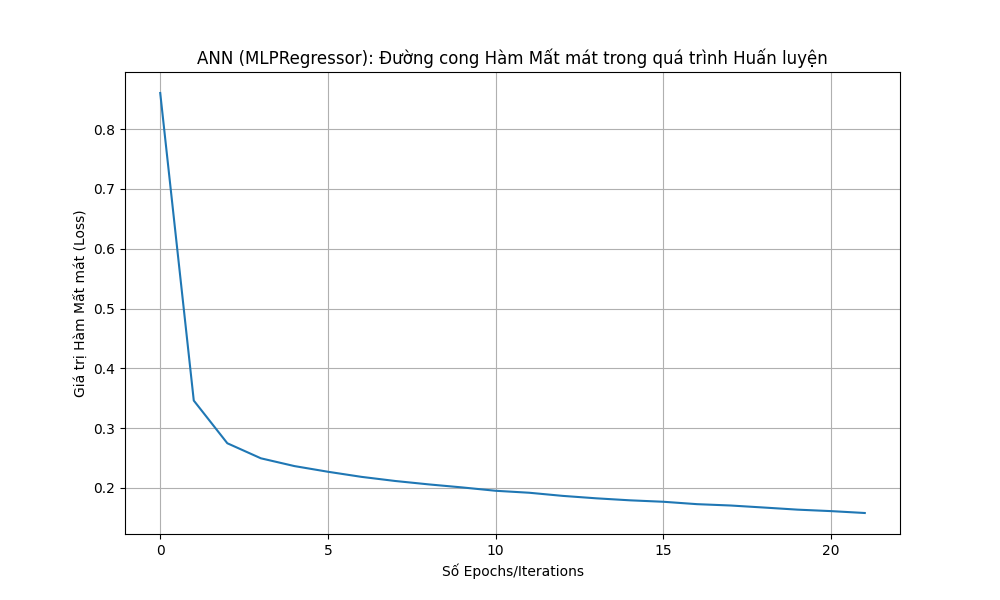
\includegraphics[width=0.8\textwidth]{Images/ann_loss_curve.png}
    \caption{Đường cong hàm mất mát (Loss Curve) của mô hình ANN trong quá trình huấn luyện. Trục hoành thể hiện số vòng lặp (epochs).}
    \label{fig:ann_loss_curve}
\end{figure}
\FloatBarrier
Hình \ref{fig:ann_loss_curve} hiển thị giá trị của hàm mất mát (loss function) qua các vòng lặp huấn luyện. Có thể thấy giá trị hàm mất mát giảm nhanh trong những vòng lặp đầu tiên và sau đó hội tụ, cho thấy mô hình đã học được từ dữ liệu. Việc mô hình dừng sớm sau 22 vòng lặp (trong khi \texttt{max\_iter=500}) là do cơ chế \texttt{early\_stopping} được kích hoạt, giúp ngăn chặn overfitting và tiết kiệm thời gian huấn luyện khi không còn sự cải thiện đáng kể trên tập validation.

\subsubsection{Tóm tắt và Nhận xét}
Mô hình Mạng Nơ-ron Nhân tạo (MLPRegressor) với cấu hình ban đầu đã cho thấy hiệu suất dự đoán khá, với $R^2 \approx 0.52$, thấp hơn một chút so với Hồi quy Tuyến tính nhưng vượt trội hơn Cây Quyết định mặc định. Điều này cho thấy ANN có khả năng mô hình hóa các mối quan hệ trong dữ liệu, nhưng cũng nhấn mạnh tầm quan trọng của việc tinh chỉnh siêu tham số (như kiến trúc mạng, tốc độ học, phương pháp điều chuẩn) để khai thác tối đa tiềm năng của mô hình. Khác với các mô hình tuyến tính hay cây quyết định, việc diễn giải trực tiếp "độ quan trọng" của từng đặc trưng trong ANN phức tạp hơn và thường đòi hỏi các kỹ thuật phân tích bổ sung (ví dụ: Permutation Importance).








\subsection{Mô hình K-Nearest Neightbors (KNN Regressor)}
\label{subsec:knn_results}

Trong phần này, nhóm em trình bày kết quả của việc áp dụng mô hình K-Láng giềng Gần nhất (K-Nearest Neighbors - KNN) Regressor để dự đoán sản lượng cây trồng. Đây là một thuật toán dựa trên khoảng cách, do đó, tương tự như mô hình ANN, các đặc trưng đầu vào đã được nhóm em chuẩn hóa bằng \texttt{StandardScaler} trước khi huấn luyện để đảm bảo tính đồng nhất về thang đo.

\subsubsection{Thông số và hiệu suất mô hình KNN}
\label{subsubsec:knn_parameters_metrics}

Mô hình KNN Regressor được nhóm em cấu hình với các tham số chính sau:
\begin{itemize}
    \item \textbf{Số láng giềng gần nhất (K - n\_neighbors):} 5
    \item \textbf{Trọng số (weights):} `distance` (các láng giềng gần hơn có ảnh hưởng lớn hơn đến dự đoán)
    \item \textbf{Metric đo khoảng cách:} `minkowski` (với p=2, tương đương khoảng cách Euclidean)
\end{itemize}

Hiệu suất của mô hình KNN trên tập kiểm tra được nhóm em đánh giá qua các chỉ số:
\begin{itemize}
    \item \textbf{Mean Absolute Error (MAE):} $0.7771$
    \item \textbf{Mean Squared Error (MSE):} $0.9200$
    \item \textbf{Root Mean Squared Error (RMSE):} $0.9592$
    \item \textbf{R-squared (R²):} $0.1284$
\end{itemize}

Giá trị $R^2 = 0.1284$ cho thấy mô hình KNN (với $K=5$ và các thiết lập như trên) chỉ giải thích được khoảng $12.84\%$ sự biến thiên của sản lượng cây trồng. Đây là một kết quả tương đối thấp so với các mô hình khác mà nhóm em đã thử nghiệm trước đó (Hồi quy Tuyến tính $R^2 \approx 0.56$, ANN $R^2 \approx 0.52$). Điều này cho thấy mô hình KNN với cấu hình hiện tại chưa thực sự phù hợp hoặc chưa khai thác tốt các mối quan hệ trong bộ dữ liệu này.

Các chỉ số sai số MAE ($0.7771$) và RMSE ($0.9592$) cũng ở mức khá cao, phản ánh độ lệch lớn hơn giữa giá trị dự đoán và giá trị thực tế so với một số mô hình trước.

\subsubsection{Trực quan hóa kết quả mô hình KNN}
\label{subsubsec:knn_visualization}

Hai biểu đồ sau giúp nhóm em đánh giá trực quan hơn về hiệu suất của mô hình KNN.

\begin{figure}[htb]
    \centering
    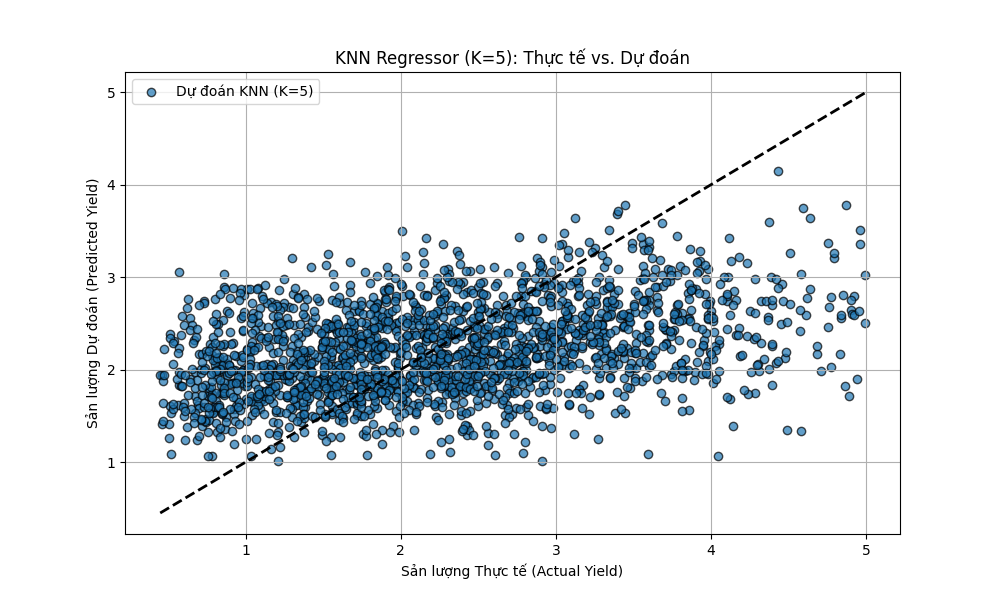
\includegraphics[width=0.8\textwidth]{Images/knn_actual_vs_predicted_plot.png}
    \caption{So sánh giá trị sản lượng thực tế và giá trị dự đoán bởi mô hình KNN (K=5) trên tập kiểm tra. Hình ảnh do nhóm em tạo ra.}
    \label{fig:knn_actual_vs_predicted}
\end{figure}

Hình \ref{fig:knn_actual_vs_predicted} minh họa sự phân tán của các điểm dự đoán so với giá trị thực tế. Nhóm em nhận thấy rằng các điểm dữ liệu phân tán khá rộng và không tập trung chặt chẽ quanh đường chéo $y=x$. Điều này trực quan hóa cho kết quả $R^2$ thấp và các chỉ số lỗi cao đã được ghi nhận.

\begin{figure}[htb]
    \centering
    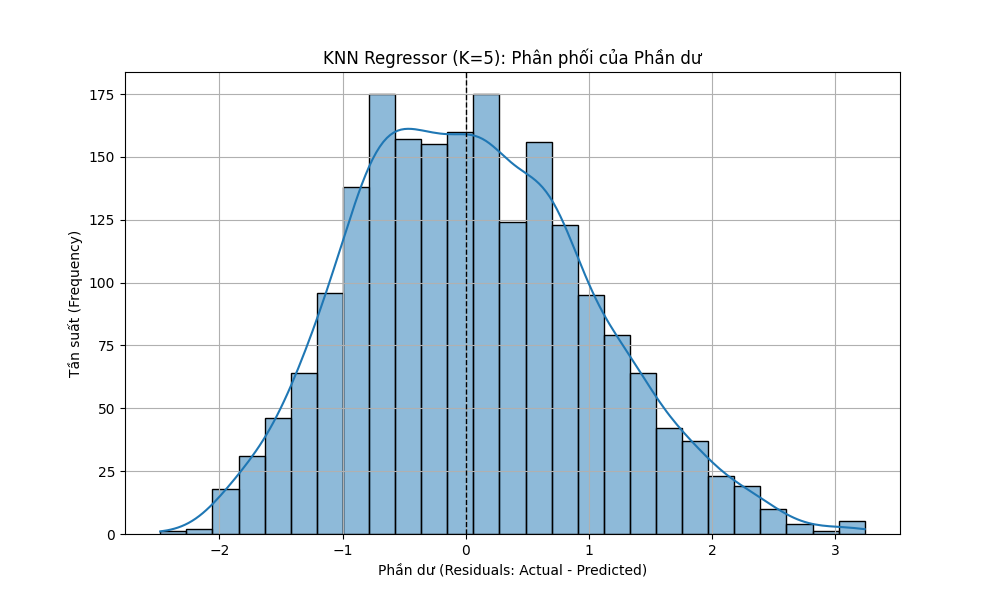
\includegraphics[width=0.8\textwidth]{Images/knn_residuals_distribution_plot.png}
    \caption{Phân phối của phần dư (Actual - Predicted) từ mô hình KNN (K=5) trên tập kiểm tra. Hình ảnh do nhóm em tạo ra.}
    \label{fig:knn_residuals_distribution}
\end{figure}

Phân phối phần dư của mô hình KNN (Hình \ref{fig:knn_residuals_distribution}) tuy có tâm lệch không quá xa 0, nhưng hình dạng của phân phối có vẻ rộng và không đều bằng một số mô hình khác, cho thấy sự biến thiên lớn trong sai số dự đoán.

\subsubsection{Tóm tắt và Nhận xét về Mô hình KNN}
Mô hình K-Láng giềng Gần nhất (KNN Regressor) với $K=5$ và các thiết lập ban đầu đã cho thấy hiệu suất dự đoán sản lượng nông nghiệp chưa cao trên bộ dữ liệu này. Kết quả $R^2$ thấp và các chỉ số lỗi MAE, RMSE cao hơn so với các mô hình như Hồi quy Tuyến tính và ANN.
Nhóm em cho rằng có một số nguyên nhân có thể dẫn đến kết quả này:
\begin{itemize}
    \item Giá trị $K=5$ có thể chưa phải là tối ưu. Việc lựa chọn $K$ phù hợp là rất quan trọng đối với KNN và thường cần được tinh chỉnh thông qua kiểm định chéo (Cross-Validation).
    \item KNN có thể nhạy cảm với "lời nguyền chiều dữ liệu" (curse of dimensionality) khi số lượng đặc trưng lớn (đặc biệt sau khi One-Hot Encoding).
    \item Bản chất của dữ liệu hoặc các mối quan hệ trong đó có thể không phù hợp với cách tiếp cận dựa trên láng giềng của KNN.
\end{itemize}
Các bước cải thiện tiềm năng cho mô hình KNN mà nhóm em có thể xem xét bao gồm việc tinh chỉnh siêu tham số $K$ một cách hệ thống, thử nghiệm các metric đo khoảng cách khác nhau, hoặc áp dụng các kỹ thuật giảm chiều dữ liệu trước khi đưa vào KNN. Tương tự như ANN, KNN cũng không cung cấp các hệ số hay độ quan trọng đặc trưng một cách trực tiếp như Hồi quy Tuyến tính hay Cây Quyết định.